%	% ****** Start of file MolecularSpinFlipLoss.tex ******
%
%
%

\documentclass[%
 reprint,
%superscriptaddress,
%groupedaddress,
%unsortedaddress,
%runinaddress,
%frontmatterverbose,
%preprint,
%showpacs,preprintnumbers,
%nofootinbib,
%nobibnotes,
%bibnotes,
 amsmath,amssymb,
 aps,
%prl,
pra,
%prb,
%rmp,
%prstab,
%prstper,
%floatfix,
]{revtex4-1}

\usepackage{graphicx}% Include figure files
\usepackage{dcolumn}% Align table columns on decimal point
\usepackage{bm}% bold math
\usepackage[hidelinks]{hyperref}% add hypertext capabilities
%\usepackage[mathlines]{lineno}% Enable numbering of text and display math
%\linenumbers\relax % Commence numbering lines
\usepackage{textcomp}

\usepackage{color}
\newcommand{\red}[1]{{\color{black} #1}}


\newcommand{\bcl}{{$B_\text{coil}$}}
\newcommand{\epb}{{$\vec{E}\s {\perp}\s\vec{B}$}}
\newcommand{\epbm}{{\vec{E}\s {\perp}\s\vec{B}}}
\newcommand{\cmnt}[1]{\ignorespaces}
\newcommand{\s}{{\nobreak\hspace{.2em}}}



\begin{document}

\title{Efficiency Boost for Stark Deceleration}%

\author{David Reens}
\thanks{dave.reens@colorado.edu.}

\author{Hao Wu}

\author{Tim Langen}%
\altaffiliation{Present Address: 5. Physikalisches Institut and Center for Integrated Quantum Science and Technology (IQST), Universit\"at Stuttgart, Pfaffenwaldring 57, 70569 Stuttgart, Germany}

\author{Jun Ye}
\affiliation{JILA, National Institute of Standards and Technology and the University of Colorado and\\ Department of Physics, University of Colorado, Boulder, Colorado 80309-0440, USA}


\date{\today}


%%%%%%%%%%%%%%%%%%%%%
%ABSTRACT
%%%%%%%%%%%%%%%%%%%%%
\begin{abstract}
Since its first realization by (Bethlem I think), Stark deceleration has unlocked incredible new opportunities for the control of molecular beams. 
Numerous trapping and collisional studies have been performed, and several important extensions to the technique have been developed. 
In particular, traveling-wave deceleration improves on the original pulsed deceleration technique by providing a true moving trap, albeit at the expense of electrode simplicity and some high voltage engineering complexities.
In this work, we introduce an alternative charging strategy that can transform a conventional pulsed electrode array into an effective moving trap decelerator.
In both simulation and experiment, the technique offers four-fold increases in molecule number with only minor adjustments to the timing of the device, and these gains persist over all final decelerated speeds.
This alternative charging strategy can also be enhanced up to nearly a ten-fold gain with some investment in high voltage technology, which we also experimentally demonstrate.
\end{abstract}


\maketitle


%%%%%%%%%%%%%%%%%%%%%%%%%%%%%%%%%
%     INTRODUCTION
%%%%%%%%%%%%%%%%%%%%%%%%%%%%%%%%%
\section{Introduction}
Stark Deceleration has been performed for this list of species and been used to study these things. In our experiment, an emphasis on trapping for longer term studies of collisional effects has enabled these other things. Higher densities are still greatly desired, and almost all studies would benefit. The measurements performed on differential scattering by Bas measure almost ppm level effects, and those on our studies can require days of averaging. Many of the enhancements offered by traveling wave type decelerators come at great costs in system complexity and high voltage engineering. For this reason it has always been of interest to improve performance, and several landmark studies have done so by different means. One technique is the appropriate combination of pulsed and traveling wave type devices, or even using traveling wave geometry with pulsed electronics. Another is the use of decelerator overtones, or of what may be thought of as a kind of undertone, both of which lead to significant improvements but at the expense of length and thermal load on switching electronics, respectively. The new technique described here makes use of alternative charging configurations, and can be achieved on conventional pulsed devices with no expenses of length or thermal load due to increased switching frequencies.

\section{Background}
One of the key motivations for improvement of the conventional pulsed decelerator operation are its well-known failings as far as phase-space stability is concerned. These have been described in terms of transverse-longitudinal couplings, small separatrix area at high phase angles, or reflection at low velocities. We introduce some new heuristics for the performance of the conventional pulsed decelerator system, borrowed from the traveling wave decelerator description. Essentially, we can also think of the pulsed decelerator as a moving trap, and instead of considering only it's phase space separatrices, consider the relevant features of this trap. These include the average depth of this effective trap as well as the worst-case depth in the case of any holes. It is found that the worst-case depth is in fact incredibly small. In particular, molecules that deviate transversely from the synchronous molecule but not longitudinally experience almost no trap at all. This can be considered the underlying reason for the transverse-longitudinal coupling problem that has been described. Such couplings are in some contexts useful for maintaining ergodicity in a trapping geometry, but with one dimension featuring a very low energy barrier to escape, they lead to loss.

\begin{figure}[t]
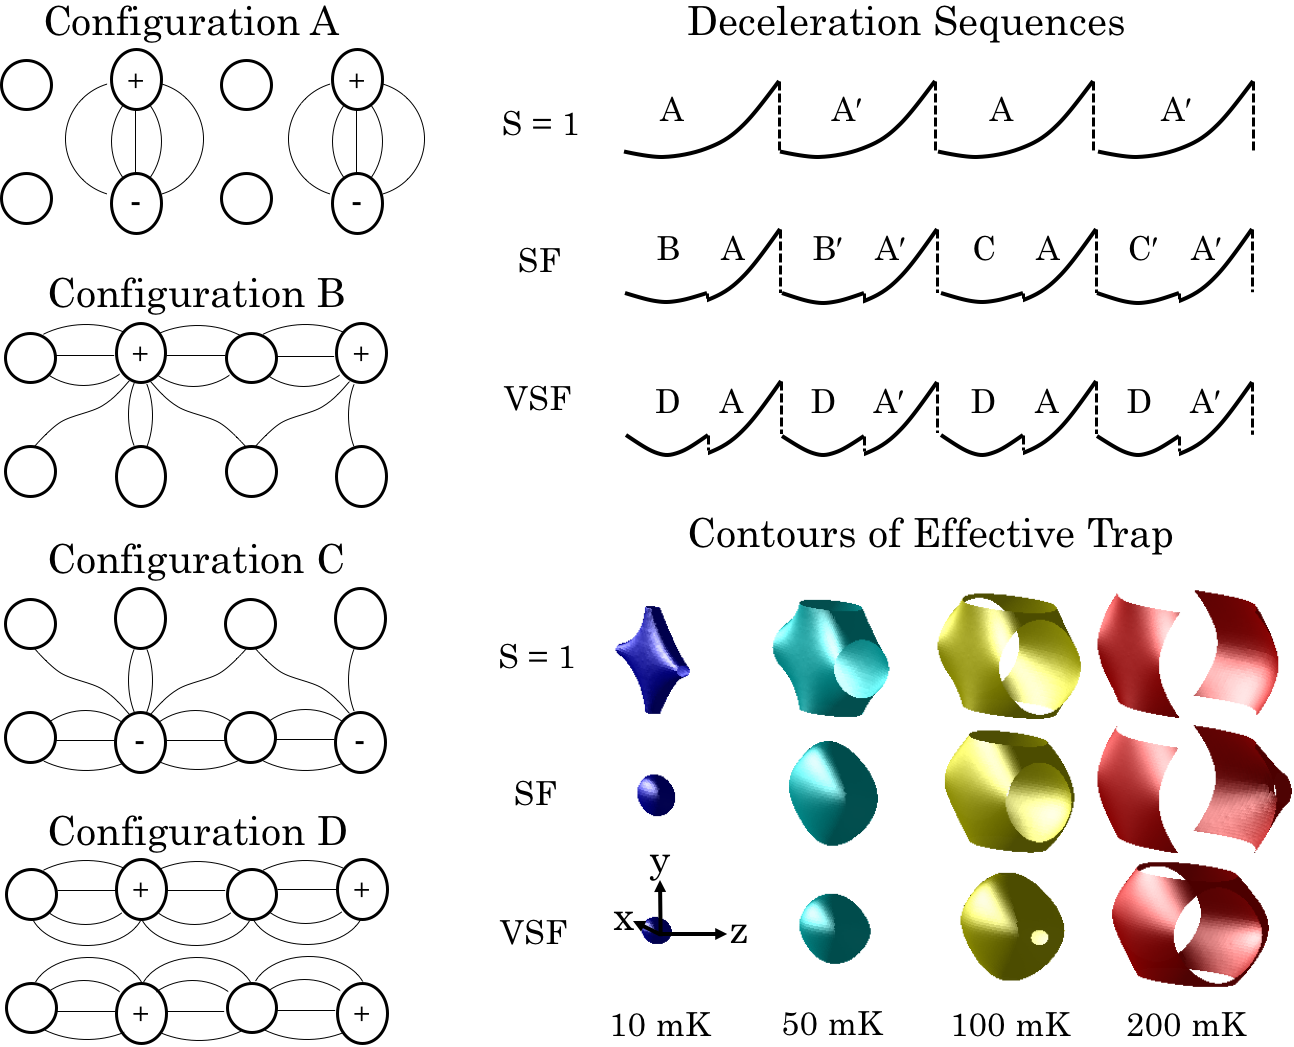
\includegraphics[width=\linewidth]{chargecartoon.png}%
\caption{
Here we show a cartoon of the field lines in normal and alternate charge configurations. Molecules experience forces towards regions of low field line density. The alternate configurations feature large transverse force between the grounded pin pair, an essentially wasted region using only normal charge configurations.
}
\label{fig:speedvary}
\end{figure}

To address this, we mix alternate charging configurations into the deceleration scheme that feature an imbalance of charge between one pin pair and the next. Typically, pin pairs are operated in a balanced bipolar manner, so that when a given pin pair is charged, one is charged positively and the other negatively. This means that the average voltage of the charged pin-pair is zero, and few field lines run toward the grounded pin-pair, which also has a zero average voltage. Once an imbalance exists, for example by charging up one pin pair to the same non-zero voltage, or simply by only charging one pin in a pair in a unipolar manner, field lines will run between pin-pairs. Near the grounded pin-pair, these field lines create a classic 2D quadrupole structure, much like the one used intentionally for trapping in our earlier paper. These alternate configurations can be implemented when the synchronous molecule is flying between the grounded pin pair, which hardly changes the longitudinal behavior of the device, but adds trap depth to the effective moving trap in the direction through the trap center in the transverse directions.

\begin{figure}[t]
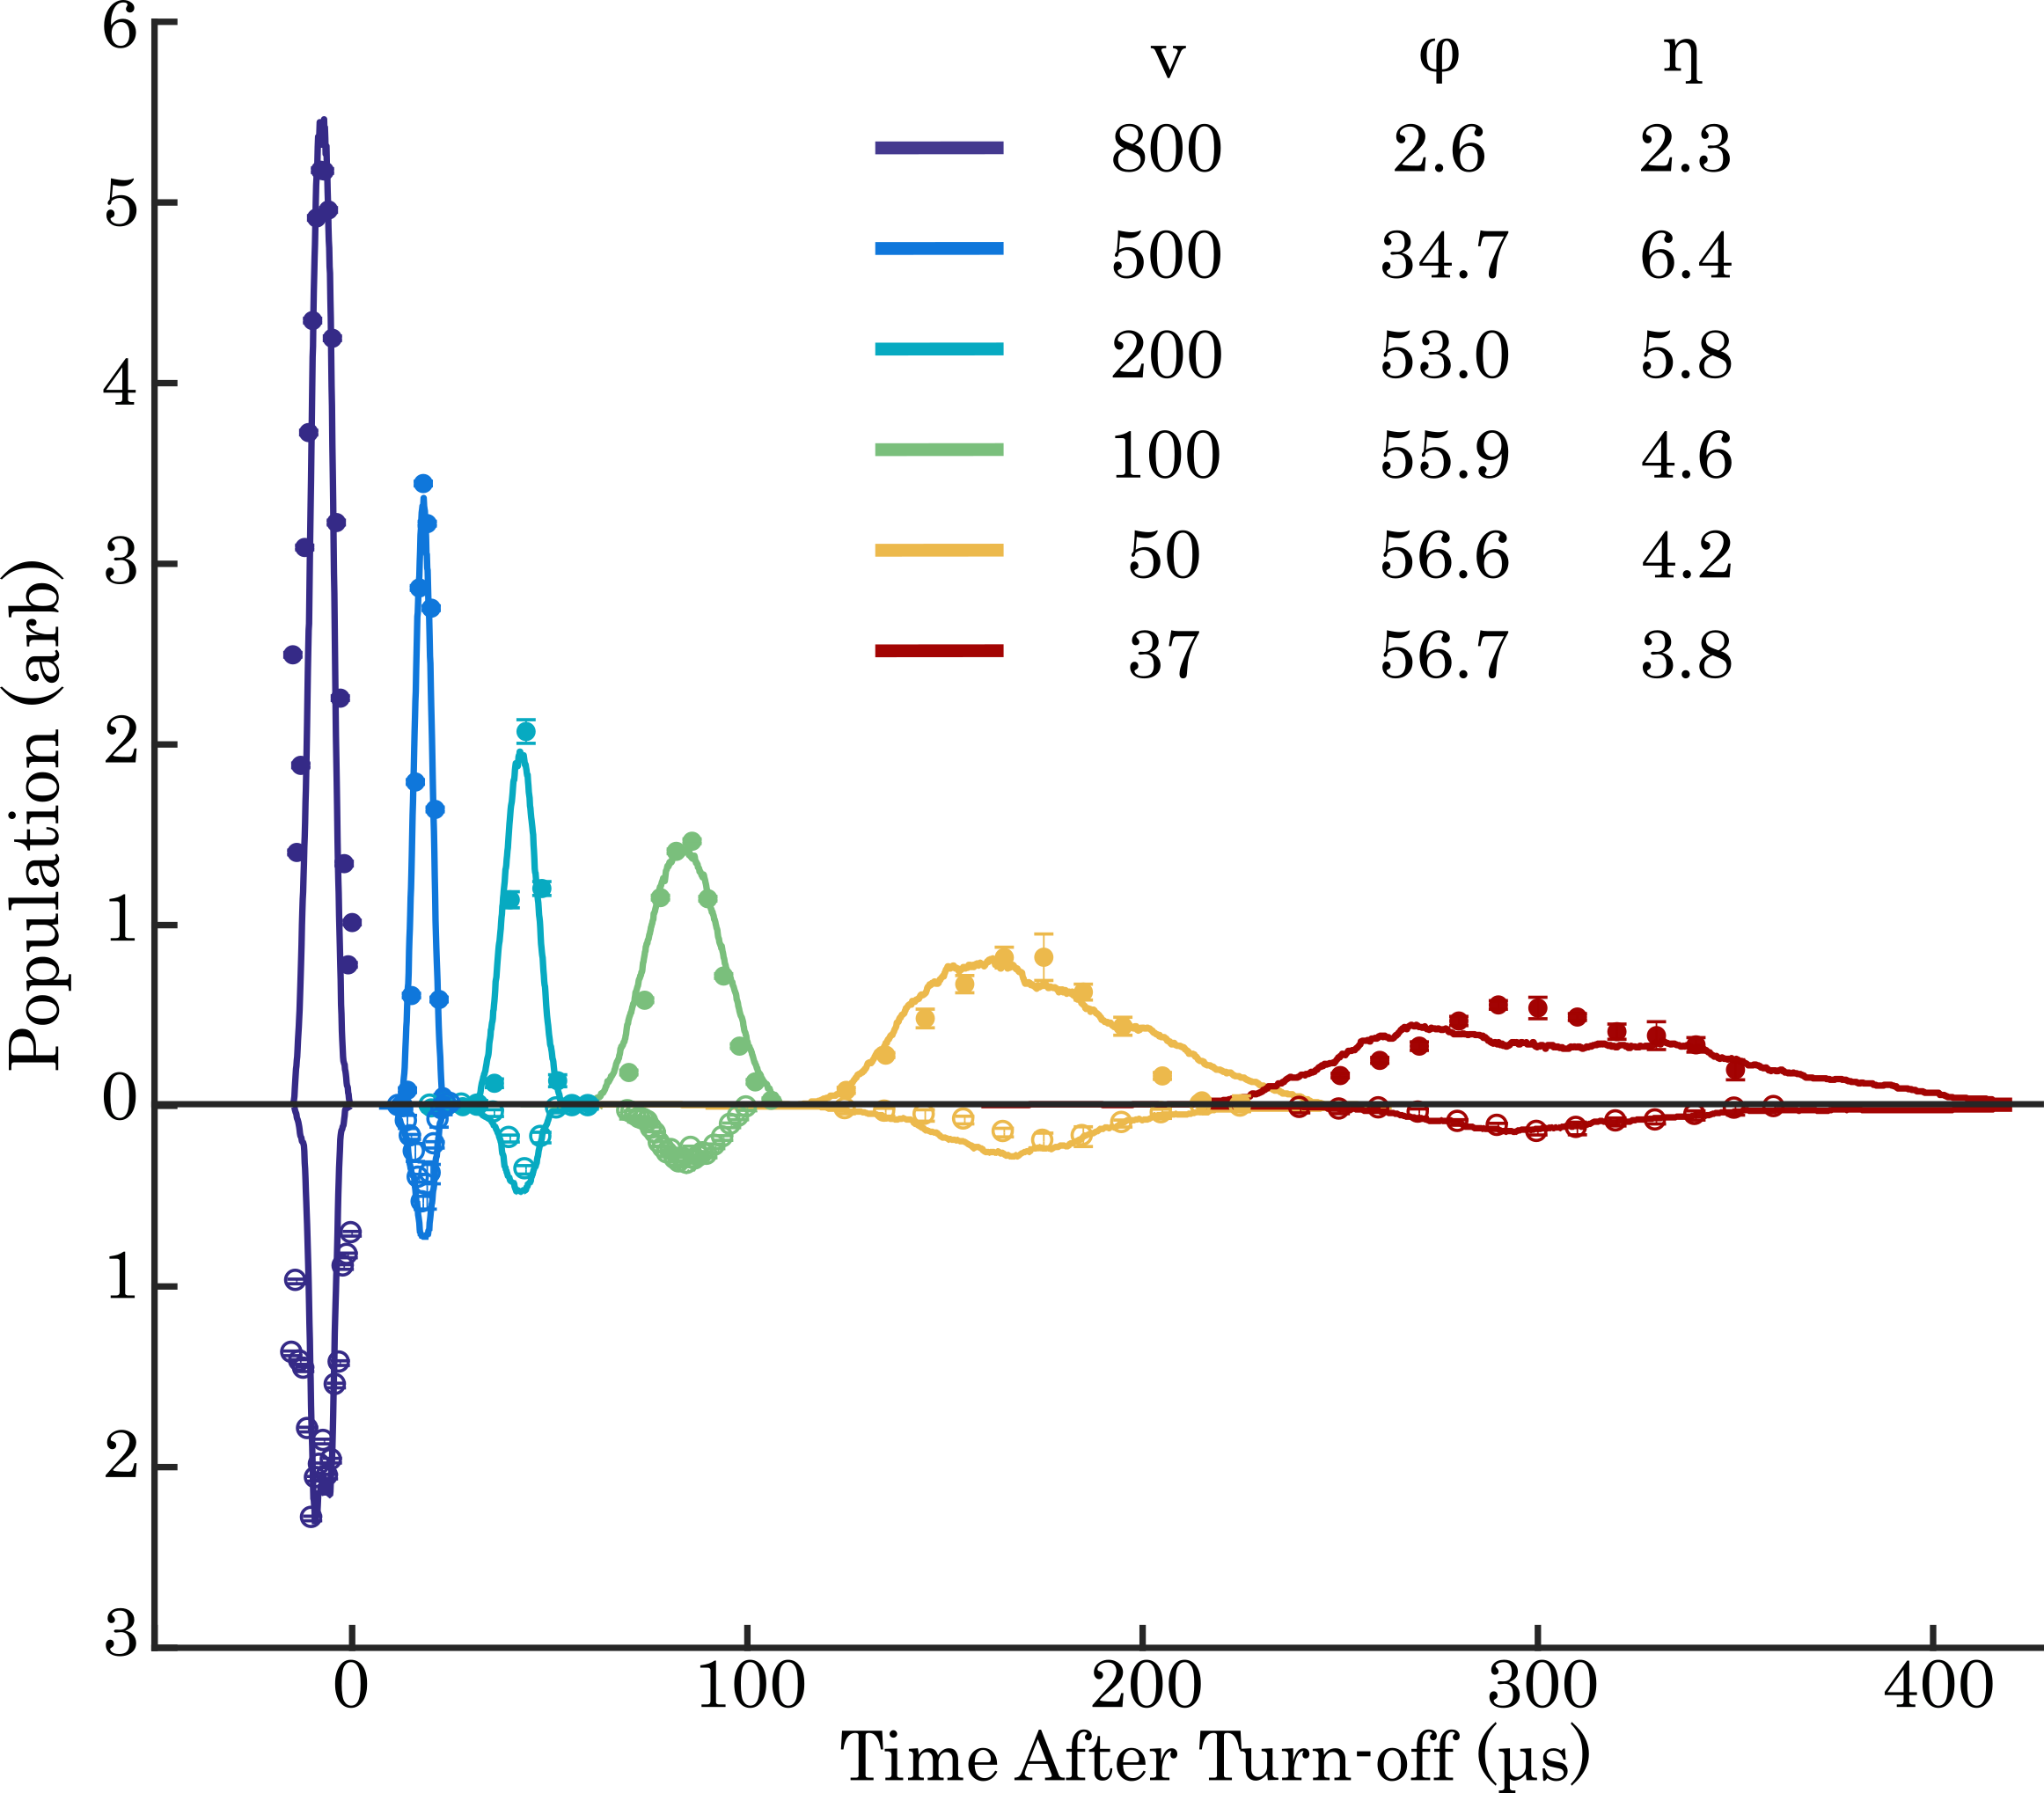
\includegraphics[width=\linewidth]{speedvary.png}%
\caption{
Wow it is so legitimate.
}
\label{fig:speedvary}
\end{figure}


\section{Results}
Our main results are shown in Fig.~\ref{fig:speedvary}. In both simulation and experiment we find fourfold enhancements across a wide range of final speeds by mixing in the alternate charging configuration of having only one pin in a pin-pair charged during part of the sequence. The slowest speeds shown are typical in a system such as ours designed to provide molecules that are one pulse away from being stopped, but the decelerator cannot serve as a trap in the same way that a true traveling wave device might since any given pin-pair only offers trapping in two dimensions. The lower panel shows the even larger gain that we observe for the more advanced technique of charging both pins in a pin-pair to the same voltage.

It is important to understand the dependence of these effects on the length of the device. Conventional schemes, and indeed our modified schemes as well, can tolerate length in accordance with the relevant time-scale for molecules at high enough orbit energies to find the low-points of the imperfect moving trap created by the deceleration sequence. In the language of Hamiltonian perturbation theory, this is known as cherenkov diffusion, and can be studied empirically by simulating very long decelerators. We do this in Fig.~\ref{fig:longtimes}. It is seen that with enough time, almost all molecules escape the conventional scheme, not surprising given the low hole depth described earlier. It is also seen that in the long-length limit, some factor of four still escape with our modified schemes. This is unavoidable for any effective trap that is deeper in some directions than in others.

\section{Discussion}
It is important to reconcile our language thus far with the notion of the phase space conservative behavior of non-dissipative Hamiltonian systems such as Stark decelerators. While it is true in theory that such systems cannot compress or dilute phase space; in practice the conserved volume can become hopelessly swirled about, so that any reasonable scientific device, which typically accepts a roughly spherical phase space volume, inevitably includes a mixture of conserved and nonconserved volumes, so that the final phase space density can be severely diluted. Simply put, a trap with a hole in it is certainly a non-dissipative Hamiltonian system, but that doesn't prevent molecules falling out of it.

\section{Conclusion}
When considering the wealth of accomplishments and the depth of achievement present in our group, it is certain that we are incredibly legitimate and that our legitimacy is in fact very solid and well founded. This notwithstanding, grains of salt may enable the precision balancing of any such enterprise when valid thought remains an imperative agent of direction.



%includes uncited bib entries
%\nocite{*}
\bibliographystyle{apsrev4-1_no_Arxiv}
\bibliography{alternatecharging}


\end{document}
%
% ****** End of file MolecularMajoranaLoss.tex ******


%% FIGURES
%Figures:
%Final Speed Panel, Sim & Expt. Add acceleration? Include extra focusing?
%1D longitudinal potential, transverse spring constant?
%2D trap contours, lab frame. Do in COMSOL.
%2D trap contours, eff frame. Gotta be Matlab. Show pins somehow.
%Phase Space Acceptance. Consider James� density coloring technique. Plot density as a function of 6D ball of increasing radius.
%Timing Diagram. Good way to show different chargings.
%Stage Number Dependence. Necessary? Interesting. Chance to work in chaos theory.
%3D trap surfaces? Need to try it to see if it is worth it.
%Is average potential same as average force?
















